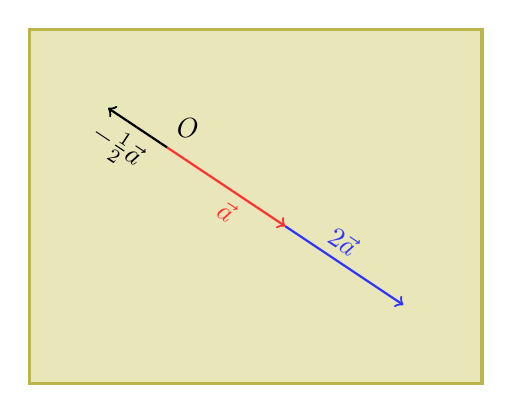
\begin{tikzpicture}
  \draw[draw = olive!60, fill = olive!20, very thick]
    (-1.75, -3) rectangle (4, 1.5);

  \draw[->, thick, color = blue!80] (1.5, -1) -- (3, -2);
  \draw[draw = none] (0, 0) -- (3, -2)
    node[pos = 0.7, above, sloped] {\textcolor{blue!80}{\(2 \vec{a}\)}};
  \draw[->, thick, color = red!80] (0, 0) -- (1.5, -1)
    node[pos = 0.6, below, sloped] {\textcolor{red!80}{\(\vec{a}\)}};
  \draw[->, thick] (0, 0) -- (-0.75, 0.5)
    node[pos = 0.6, below, sloped] {\(-\frac{1}{2} \vec{a}\)};

  \draw (0, 0) node[above right] {\(O\)};
  \point{0, 0};
\end{tikzpicture}
